\documentclass[aspectratio=169,11pt]{beamer}

% =================================================
% PACKAGES
% =================================================
\usepackage{graphicx}
\usepackage{tikz}
\usetikzlibrary{positioning,arrows.meta}
\usepackage{xcolor}
\usepackage{booktabs}
\usepackage{tabularx}
\usepackage{array}
\usepackage{ragged2e}

% =================================================
% COLORS
% =================================================
\definecolor{GEUBlue}{RGB}{20,55,105}
\definecolor{GEULightBlue}{RGB}{238,244,251}
\definecolor{GEUGrey}{RGB}{90,90,90}
\definecolor{GEULightGrey}{RGB}{245,246,248}

% =================================================
% THEME
% =================================================
\usetheme{default}

\setbeamertemplate{navigation symbols}{}

\setbeamertemplate{blocks}[rounded][shadow=false]

\setbeamercolor{normal text}{fg=black,bg=white}
\setbeamercolor{frametitle}{fg=GEUBlue}
\setbeamercolor{structure}{fg=GEUBlue}
\setbeamercolor{block title}{fg=GEUBlue,bg=GEULightBlue}
\setbeamercolor{block body}{fg=black,bg=GEULightBlue}

\setbeamerfont{frametitle}{size=\Large,series=\bfseries}

% =================================================
% LOGO
% =================================================
% Put graphicera_logo.png in the same folder as this .tex file
\newcommand{\GEULogo}{graphicera_logo.png}

% =================================================
% HEADER
% =================================================
\setbeamertemplate{headline}{%
  \begin{tikzpicture}[remember picture,overlay]
    \node[
      anchor=north east,
      xshift=-0.30cm,
      yshift=-0.12cm
    ]
    at (current page.north east)
    {\includegraphics[height=0.62cm]{\GEULogo}};
  \end{tikzpicture}
  \vspace{0.72cm}
}

% =================================================
% FRAME TITLE
% =================================================
\setbeamertemplate{frametitle}{%
  \vspace{0.03cm}
  \insertframetitle\par
  \vspace{0.04cm}
  \textcolor{GEUBlue}{\rule{\textwidth}{0.9pt}}
  \vspace{0.03cm}
}

% =================================================
% FOOTER
% =================================================
\setbeamertemplate{footline}{%
  \leavevmode
  \hbox{%
  \begin{beamercolorbox}[
    wd=.82\paperwidth,
    ht=0.32cm,
    dp=0.10cm,
    leftskip=.3cm
  ]{author in head/foot}
    \tiny Department of Computer Science \& Engineering
    | Graphic Era (Deemed to be University)
  \end{beamercolorbox}%
  \begin{beamercolorbox}[
    wd=.18\paperwidth,
    ht=0.32cm,
    dp=0.10cm,
    rightskip=.3cm
  ]{date in head/foot}
    \hfill\tiny\insertframenumber/\inserttotalframenumber
  \end{beamercolorbox}}
}

% =================================================
% CUSTOM COMMAND
% =================================================
\newcommand{\smallnote}[1]{
\vspace{0.08cm}
{\scriptsize\color{GEUGrey}#1}
}

% =================================================
% TITLE INFORMATION
% =================================================
\title{
\textbf{Project-Based Learning}\\[2mm]
\large Phase-I Evaluation
}

\author{
\textbf{Smart Emergency Response System}\\
Team ID: XXXX
}

\institute{
Department of Computer Science \& Engineering\\
Graphic Era (Deemed to be University), Dehradun
}

\date{Academic Session 2026--27}


% =================================================
% DOCUMENT
% =================================================
\begin{document}


% =================================================
% SLIDE 1
% =================================================
\begin{frame}[plain]

\begin{tikzpicture}[remember picture,overlay]

% Top blue line
\draw[
  GEUBlue,
  line width=3pt
]
(current page.north west) --
(current page.north east);

% Logo
\node[
  anchor=north east,
  xshift=-0.45cm,
  yshift=-0.35cm
]
at (current page.north east)
{\includegraphics[height=1.0cm]{graphicera_logo.png}};

% Main title
\node[
  align=center,
  text width=.84\paperwidth
]
at ([yshift=.25cm]current page.center)
{
{\color{GEUBlue}
\fontsize{26}{30}\selectfont
\bfseries PROJECT-BASED LEARNING}\\[3mm]

{\fontsize{18}{22}\selectfont
PHASE-I EVALUATION}\\[7mm]

{\color{GEUGrey}
\Large\bfseries
Smart Emergency Response System}\\[3mm]

{\color{GEUBlue}
\normalsize Team ID: DSCPP-III-2026-T232}
};

% Institute information
\node[
  align=center,
  anchor=south,
  yshift=.42cm
]
at (current page.south)
{
\bfseries Department of Computer Science \& Engineering\\
Graphic Era (Deemed to be University), Dehradun\\[-1mm]
\scriptsize Academic Session 2026--27
};

\end{tikzpicture}

\end{frame}


% =================================================
% SLIDE 2
% =================================================
\begin{frame}{Team \& Mentor Details}

\begin{columns}[T,totalwidth=\textwidth]

% -------------------------------------------------
% LEFT COLUMN
% -------------------------------------------------
\column{.48\textwidth}

\begin{block}{Team Information}

\begin{tabular}{@{}ll@{}}

\textbf{Team ID:} & DSCPP-III-2026-T232\\
\textbf{Semester:} & 3rd\\
\textbf{Section:} & DS1, ML1, B, DS2   \\
\textbf{Domain:} & DSA / C++

\end{tabular}

\end{block}

% -------------------------------------------------
% RIGHT COLUMN
% -------------------------------------------------
\column{.48\textwidth}
\begin{block}{Team Members}
1.\quad \placeholder{Sambhawi Pandey -- 2510380216}\\
2.\quad \placeholder{Atharv Rawat -- 2510370380}\\
3.\quad \placeholder{Aayush Lalotra -- 2510012608}\\
4.\quad \placeholder{Shivam Garg -- 2510386512}
\end{block}
\end{columns}
\vspace{2mm}
\begin{block}{Mentor}
\placeholder{Mr.Rohan Verma}
\hfill
\textbf{Interactions completed: 3} 
\end{block}
\end{frame}

% =================================================
% SLIDE 3
% =================================================
\begin{frame}{Problem Statement \& Motivation}

\begin{block}{Problem Statement}

Emergencies such as road accidents, fires and medical incidents
may occur simultaneously while emergency resources are limited.
Manual prioritization and resource allocation can delay response.

\end{block}

\vspace{2mm}

\begin{columns}[T,totalwidth=\textwidth]

% -------------------------------------------------
% MOTIVATION
% -------------------------------------------------
\column{.48\textwidth}

\textbf{\color{GEUBlue}Motivation}

\begin{itemize}
\itemsep2pt

\item Faster emergency prioritization
\item Efficient resource allocation
\item Shortest route selection
\item Handling multiple emergencies

\end{itemize}

% -------------------------------------------------
% TARGET USERS
% -------------------------------------------------
\column{.48\textwidth}

\textbf{\color{GEUBlue}Target Users / Stakeholders}

\begin{itemize}
\itemsep2pt

\item Emergency operators / dispatchers
\item Ambulance and response teams
\item Hospitals, police and fire services
\item Emergency reporting users

\end{itemize}

\end{columns}

\vfill

\end{frame}


% =================================================
% SLIDE 4
% =================================================
\begin{frame}{Objectives}
\textbf{\color{GEUBlue}Project Objectives}
\vspace{2mm}
\begin{enumerate}\itemsep5pt
\item \placeholder{Develop an emergency reporting and management system.}
\item \placeholder{Categorize and prioritize emergencies using severity and Priority Queue.}
\item \placeholder{Manage emergency resources such as ambulances efficiently.}
\item \placeholder{Model roads and calculate shortest routes using Graphs and Dijkstra’s Algorithm.}
\item \placeholder{Apply DSA and OOP in C++ and test the system with different emergency scenarios.}
\end{enumerate}
\vfill
\begin{center}
\colorbox{GEULightBlue}{\parbox{.80\textwidth}{\centering
\textbf{Key Objective:} \placeholder{Emergency response system that prioritizes incidents, manages resources, and finds optimal routes}}}
\end{center}
\end{frame}


% =================================================
% SLIDE 5
% =================================================
\begin{frame}{Proposed Solution}

\begin{columns}[T,totalwidth=\textwidth]

% -------------------------------------------------
% APPROACH
% -------------------------------------------------
\column{.48\textwidth}

\textbf{\color{GEUBlue}Proposed Approach}

\begin{enumerate}
\itemsep3pt

\item Emergency Data Collection
\item Emergency Validation
\item Severity-Based Prioritization
\item Resource Allocation
\item Shortest Route Calculation
\item Dispatch \& Status Update

\end{enumerate}

% -------------------------------------------------
% FEATURES
% -------------------------------------------------
\column{.48\textwidth}

\textbf{\color{GEUBlue}Key Features}

\begin{itemize}
\itemsep3pt

\item Emergency Management
\item Priority Queue / Heap
\item Ambulance Management
\item Graph + Dijkstra
\item Status Tracking
\item Searching \& Sorting

\end{itemize}

\end{columns}

\vfill


\end{frame}


% =================================================
% SLIDE 6
% =================================================
\begin{frame}{Integration of PBL Course Concepts}

\scriptsize

\begin{center}

\renewcommand{\arraystretch}{1.45}

\begin{tabularx}{.96\textwidth}
{@{}>{\bfseries}p{3.2cm}X p{3.0cm}@{}}

\toprule

Course & Concepts Applied & Project Module\\

\midrule

Data Structures in C
&
Arrays, Linked Lists, Queues, Priority Queue,
Heaps, Graphs, Searching \& Sorting
&
Emergency \& Resource Management
\\

OOPS in C++
&
Classes, Objects, Encapsulation,
Abstraction, Constructors and OOP Concepts
&
Emergency \& Ambulance Modules
\\

\bottomrule

\end{tabularx}

\end{center}

\vfill

\begin{center}

\colorbox{GEULightBlue}{
\parbox{.86\textwidth}{
\centering
\textbf{Core Integration:}
Data Structures provide the core algorithms and data handling,
while C++ is used to implement the complete system.
}}

\end{center}

\end{frame}


% =================================================
% SLIDE 7
% =================================================
\begin{frame}{System Architecture / Workflow}

\begin{center}

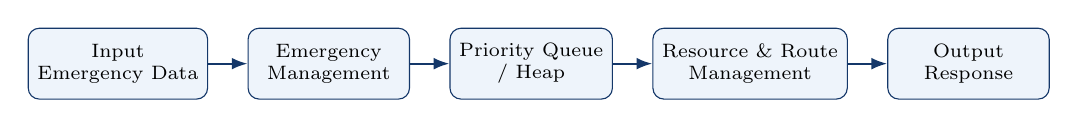
\begin{tikzpicture}[
node distance=5mm,
box/.style={
rectangle,rounded corners,draw=GEUBlue,fill=GEULightBlue,
minimum width=2.05cm,minimum height=9mm,
align=center,font=\scriptsize
},
arrow/.style={-{Latex[length=2mm]},thick,draw=GEUBlue}
]

\node[box] (a) {Input\\Emergency Data};

\node[box,right=of a] (b) {Emergency\\Management};

\node[box,right=of b] (c) {Priority Queue\\/ Heap};

\node[box,right=of c] (d) {Resource \& Route\\Management};

\node[box,right=of d] (e) {Output\\Response};

\draw[arrow] (a)--(b);
\draw[arrow] (b)--(c);
\draw[arrow] (c)--(d);
\draw[arrow] (d)--(e);

\end{tikzpicture}

\end{center}

\vspace{3mm}

\begin{columns}[T,totalwidth=\textwidth]

\column{.48\textwidth}

\textbf{\color{GEUBlue}Major Components}

\begin{itemize}\itemsep1pt
\small
\item Emergency Management
\item Priority Queue / Heap
\item Resource Management
\item Graph + Dijkstra's Algorithm
\end{itemize}

\column{.48\textwidth}

\textbf{\color{GEUBlue}Data / Control Flow}

\begin{itemize}\itemsep1pt
\scriptsize
\item Emergency data is registered and categorized by severity.
\item Priority Queue prioritizes critical emergencies.
\item Available resources are selected and shortest routes are calculated.
\item System displays assigned resource, route and response status.
\end{itemize}

\end{columns}

\end{frame}


% =================================================
% SLIDE 8
% =================================================
\begin{frame}{Technology Stack \& Methodology}

\begin{columns}[T,totalwidth=\textwidth]

% -------------------------------------------------
% TECHNOLOGY STACK
% -------------------------------------------------
\column{.48\textwidth}
\vspace{-8mm}
\begin{block}{Technology Stack}

\begin{itemize}
\itemsep3pt

\item Programming Language: \textbf{C++}
\item Paradigm: \textbf{Object-Oriented Programming}
\item Data Structures: \textbf{Queue, Heap, Graph}
\item Algorithms: \textbf{Dijkstra, Searching, Sorting}
\item Development Tool: \textbf{Visual Studio Code}
\item Version Control: \textbf{Git / GitHub}

\end{itemize}

\end{block}

% -------------------------------------------------
% METHODOLOGY
% -------------------------------------------------
\column{.48\textwidth}
\vspace{-8mm}
\begin{block}{Development Methodology}

\begin{center}
\vspace{2mm}

\includegraphics[width=0.95\linewidth,height=5.5cm,keepaspectratio]{development.jpg}

\vspace{2mm}
\end{center}

\end{block}

\end{columns}

\vfill

\begin{center}


\end{center}

\end{frame}

% =================================================
% SLIDE 9
% =================================================
\begin{frame}{Initial Progress \& Team Contribution}

\begin{columns}[T,totalwidth=\textwidth]

% -------------------------------------------------
% PROGRESS
% -------------------------------------------------
\column{.44\textwidth}

\textbf{\color{GEUBlue}Progress Achieved}

\begin{itemize}
\itemsep3pt

\item Background / literature study completed
\item Requirements identified
\item System architecture prepared
\item Initial modules planned
\item Data requirements identified

\end{itemize}

% -------------------------------------------------
% CONTRIBUTION
% -------------------------------------------------
\column{.52\textwidth}

\textbf{\color{GEUBlue}Individual Contribution}

\vspace{2mm}

\scriptsize

\begin{tabularx}{\textwidth}
{@{}p{1.6cm}p{2.0cm}X@{}}

\toprule

Member & Role & Contribution\\

\midrule

Sambhawi Pandey & Team Lead &
Planning, coordination and system design
\\

Atharv Rawat & Developer &
Core C++ modules and algorithms
\\

Aayush Lalotra & DS / Testing &
Data structures and test cases
\\

Shivam Garg & Developer/ Docs &
Implementation support and documentation
\\

\bottomrule

\end{tabularx}

\end{columns}

\end{frame}


% =================================================
% SLIDE 10
% =================================================
% =================================================
% ROADMAP & EXPECTED OUTCOMES
% =================================================

\begin{frame}{Roadmap \& Expected Outcomes}

\begin{columns}[T,totalwidth=\textwidth]

% -------------------------------------------------
% LEFT COLUMN
% -------------------------------------------------
\column{.47\textwidth}

\textbf{\color{GEUBlue}Roadmap}

\begin{enumerate}
\itemsep3pt

\item Phase-I: Proposal \& Design
\item Phase-II: Development
\item Phase-III: Final Implementation

\end{enumerate}

% -------------------------------------------------
% EXPECTED OUTCOMES
% -------------------------------------------------

\vspace{2mm}

\textbf{\color{GEUBlue}Expected Outcomes}

\begin{itemize}
\itemsep2pt

\item Emergency prioritization
\item Resource allocation
\item Shortest route calculation
\item Emergency status tracking
\item Testable system results

\end{itemize}

\end{columns}

\end{frame}


% =================================================
% REFERENCES
% =================================================

\begin{frame}{References}

\begin{enumerate}
\itemsep3pt

\item ``Ambulance Routing for Disaster Response with Patient Groups,''
\textit{Computers \& Operations Research}, vol. 56, pp. 120--133, 2015.

\item ``Integrating GIS, GPS and GSM Technologies for the Effective Management of Ambulances,''
\textit{International Journal of Medical Informatics}.

\item ``A Systematic Review of Route Optimisation and Pre-emption Methods for Emergency Vehicles,''
\textit{Transport Reviews}, vol. 40, no. 1, pp. 35--53, 2020.


\end{enumerate}

\vfill

\begin{center}

\colorbox{GEUBlue}{
\parbox{0.78\textwidth}{
\centering
\color{white}
\textbf{\large Thank You}\\[1mm]
Questions \& Suggestions
}}

\end{center}

\end{frame}


% =================================================
% END
% =================================================
\end{document}